\item (16 marks)  Here is  a list  of  five propositional  forms  and three  circuits. This  list
  contains four pairs of logically equivalent entries (we will say a circuit is equivalent
  to a propositional form  if the propositional form describes the  value of the circuit's
  output for all possible combinations of input values). For instance, maybe $A \equiv B$,
  $C \equiv D$, $E  \equiv F$ and $G \equiv H$). First determine  the four pairs, and then
  prove for each  pair that one element of  the pair is logically equivalent  to the other
  one.
  \begin{enumerate}[(A)]
  \item $a \land \lnot b$.
  \item $(a \xor b) \lor (b \xor c)$.
  \item $\lnot ((a \implies c) \wedge \lnot (c \implies b)$.
  \item $(a \implies (\lnot b \land c)) \land (\lnot b \implies c)$.
  \item $(\lnot a \lor \lnot b) \land (\lnot a \lor c) \land (b \lor c)$.
  \item \leavevmode\lower45pt\hbox{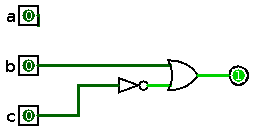
\includegraphics[scale=0.5]{ass1-q3f.png}}
  \item \leavevmode\lower45pt\hbox{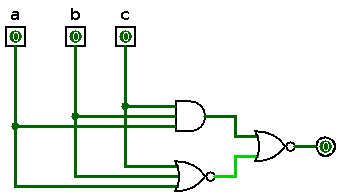
\includegraphics[scale=0.5]{ass1-q3g.png}}
  \item \leavevmode\lower45pt\hbox{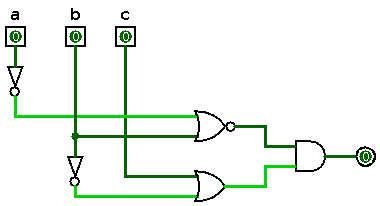
\includegraphics[scale=0.5]{ass1-q3h.png}}
  \end{enumerate}

  You are  allowed to use truth  tables to figure  out the equivalences; however  at least
  three of your proofs must use a  sequence of known logical equivalences (see Epp-4 table
  2.1.1, Epp-3  table 1.1.1, Rosen-6 table  6 in section  1.2, Rosen-7 table 6  in section
  1.3, or Dave's excellent formula sheet; you can also assume that $x \implies y \equiv \;
  {\lnot x \vee y}$ and that $x \oplus y \equiv (x \lor y)\, \land \sim\! (x \land y) \equiv
  (\lnot x \land y) \lor (x \land \lnot y)$. The fourth proof can use either a sequence of
  known logical equivalences, or a truth table.

  Hint: you might want to translate the  circuits into formulas that mirror exactly as the
  circuit is implemented, before using any logical equivalence rules.
  \newpage
\begin{enumerate}
\item \LARGE\underline{~~~~~~~~~}$\equiv$\underline{~~~~~~~~~~}\\

\begin{tabular}{rcl|l}
~~~~~~expression 1 & & expression 2~~~~~~ & reason \\
\hline
& $\equiv$ & & ~~~~~~~~~~~~~~~~~~~~~~~\\
\hline
& $\equiv$ & & ~~~~~~~~~~~~~~~~~~~~~~~\\
\hline
& $\equiv$ & & ~~~~~~~~~~~~~~~~~~~~~~~\\
\hline
& $\equiv$ & & ~~~~~~~~~~~~~~~~~~~~~~~\\
\hline
& $\equiv$ & & ~~~~~~~~~~~~~~~~~~~~~~~\\
\hline
& $\equiv$ & & ~~~~~~~~~~~~~~~~~~~~~~~\\
\hline
& $\equiv$ & & ~~~~~~~~~~~~~~~~~~~~~~~\\
\hline
& $\equiv$ & & ~~~~~~~~~~~~~~~~~~~~~~~\\
\hline
& $\equiv$ & & ~~~~~~~~~~~~~~~~~~~~~~~\\
\hline
& $\equiv$ & & ~~~~~~~~~~~~~~~~~~~~~~~\\
\hline
\end{tabular}
\large
\newpage
\item \LARGE\underline{~~~~~~~~~}$\equiv$\underline{~~~~~~~~~~}\\

\begin{tabular}{rcl|l}
~~~~~~expression 1 & & expression 2~~~~~~ & reason \\
\hline
& $\equiv$ & & ~~~~~~~~~~~~~~~~~~~~~~~\\
\hline
& $\equiv$ & & ~~~~~~~~~~~~~~~~~~~~~~~\\
\hline
& $\equiv$ & & ~~~~~~~~~~~~~~~~~~~~~~~\\
\hline
& $\equiv$ & & ~~~~~~~~~~~~~~~~~~~~~~~\\
\hline
& $\equiv$ & & ~~~~~~~~~~~~~~~~~~~~~~~\\
\hline
& $\equiv$ & & ~~~~~~~~~~~~~~~~~~~~~~~\\
\hline
& $\equiv$ & & ~~~~~~~~~~~~~~~~~~~~~~~\\
\hline
& $\equiv$ & & ~~~~~~~~~~~~~~~~~~~~~~~\\
\hline
& $\equiv$ & & ~~~~~~~~~~~~~~~~~~~~~~~\\
\hline
& $\equiv$ & & ~~~~~~~~~~~~~~~~~~~~~~~\\
\hline
& $\equiv$ & & ~~~~~~~~~~~~~~~~~~~~~~~\\
\hline
& $\equiv$ & & ~~~~~~~~~~~~~~~~~~~~~~~\\
\hline
& $\equiv$ & & ~~~~~~~~~~~~~~~~~~~~~~~\\
\hline
& $\equiv$ & & ~~~~~~~~~~~~~~~~~~~~~~~\\
\hline
& $\equiv$ & & ~~~~~~~~~~~~~~~~~~~~~~~\\
\hline
& $\equiv$ & & ~~~~~~~~~~~~~~~~~~~~~~~\\
\hline
& $\equiv$ & & ~~~~~~~~~~~~~~~~~~~~~~~\\
\hline
& $\equiv$ & & ~~~~~~~~~~~~~~~~~~~~~~~\\
\hline
& $\equiv$ & & ~~~~~~~~~~~~~~~~~~~~~~~\\
\hline
& $\equiv$ & & ~~~~~~~~~~~~~~~~~~~~~~~\\
\hline
\end{tabular}\\
\large
\newpage
\item \LARGE\underline{~~~~~~~~~}$\equiv$\underline{~~~~~~~~~~}\\

\begin{tabular}{rcl|l}
~~~~~~expression 1 & & expression 2~~~~~~ & reason \\
\hline
& $\equiv$ & & ~~~~~~~~~~~~~~~~~~~~~~~\\
\hline
& $\equiv$ & & ~~~~~~~~~~~~~~~~~~~~~~~\\
\hline
& $\equiv$ & & ~~~~~~~~~~~~~~~~~~~~~~~\\
\hline
& $\equiv$ & & ~~~~~~~~~~~~~~~~~~~~~~~\\
\hline
& $\equiv$ & & ~~~~~~~~~~~~~~~~~~~~~~~\\
\hline
& $\equiv$ & & ~~~~~~~~~~~~~~~~~~~~~~~\\
\hline
& $\equiv$ & & ~~~~~~~~~~~~~~~~~~~~~~~\\
\hline
& $\equiv$ & & ~~~~~~~~~~~~~~~~~~~~~~~\\
\hline
& $\equiv$ & & ~~~~~~~~~~~~~~~~~~~~~~~\\
\hline
& $\equiv$ & & ~~~~~~~~~~~~~~~~~~~~~~~\\
\hline
& $\equiv$ & & ~~~~~~~~~~~~~~~~~~~~~~~\\
\hline
& $\equiv$ & & ~~~~~~~~~~~~~~~~~~~~~~~\\
\hline
& $\equiv$ & & ~~~~~~~~~~~~~~~~~~~~~~~\\
\hline
& $\equiv$ & & ~~~~~~~~~~~~~~~~~~~~~~~\\
\hline
& $\equiv$ & & ~~~~~~~~~~~~~~~~~~~~~~~\\
\hline
& $\equiv$ & & ~~~~~~~~~~~~~~~~~~~~~~~\\
\hline
& $\equiv$ & & ~~~~~~~~~~~~~~~~~~~~~~~\\
\hline
& $\equiv$ & & ~~~~~~~~~~~~~~~~~~~~~~~\\
\hline
& $\equiv$ & & ~~~~~~~~~~~~~~~~~~~~~~~\\
\hline
& $\equiv$ & & ~~~~~~~~~~~~~~~~~~~~~~~\\
\hline
\end{tabular}
\large
\newpage
\item \LARGE\underline{~~~~~~~~~}$\equiv$\underline{~~~~~~~~~~}\\
\newpage
\end{enumerate}